\section{Convoluzione}
La convoluzione è un operatore matematico che descrive l'interazione tra il segnale e il filtro, e ne osserva il comportamento durante il movimento nello spazio. Si definisce nel dominio continuo fra due funzioni $g(x)$ e $f(x)$ tale che:
\begin{enumerate}
	\item L'asse di rappresentazione di uno dei due assi è invertita, $g(t) \rightarrow g(-t)$;
	\item Il segnale invertito viene fatto traslare tra $\infty$ e $-\infty$;
	\item Per ogni traslazione si calcola il prodotto tra il segnale traslato e l'altro non traslato;
	\item Si calcola l'area del prodotto, cioè la somma degli infiniti prodotti composti da una funzione che scorre e una statica.
\end{enumerate}
La convoluzione è l'operatore $*$ con cui sono descritti i filtraggi lineari nel dominio spaziale, cioè l'applicazione di una funzione $f$ a una funzione $h$ chiamata filtro (filter kernel, descrive il sistema) per ogni valore di $x$. Gode della proprietà commutativa.
$$g * f = \int_{x=-\infty}^{\infty}g(x - s)f(s) ds$$
Nel caso di funzioni discrete, essa è definita come una somma di prodotti tra gli elementi di $f$ e i coefficienti di $h$, con funzioni che sono in realtà sequenze:
$$g(x) = \sum_{m}f(m)h(x - m)$$

\begin{wrapfigure}{R}{0.3\textwidth}
	\vspace{-15pt}
	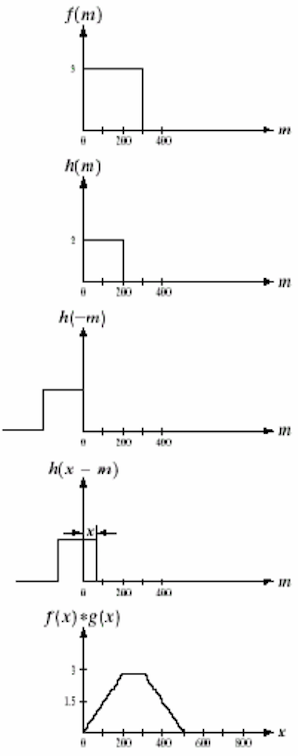
\includegraphics[width=0.3\textwidth]{Lezioni/Immagini/convoluzione}
	\vspace{-15pt}
\end{wrapfigure}

Se i segnali non si sovrappongono, la somma dei loro prodotti è 0. Quando iniziano a sovrapporsi progressivamente, se sono positivi, i valori crescono fino a raggiungere un massimo, per poi diminuire.

La lunghezza finale della funzione ottenuta dipende dai due segnali che la compongono: assumendo che non ci siano valori nulli, con $A$ punti di $f(m)$ e $B$ di $h(-m)$ si ha $g(x)$ con $A + B - 1$ punti.

Applicando la definizione di trasformata di Fourier, si può dimostrare il fondamentale teorema della convoluzione. La trasformata della convoluzione di due funzioni è il prodotto delle trasformate delle due funzioni: 
$$G(u) = \digamma[g(x)] = \digamma[f(x) * h(x)] = F(u)H(u)$$
La somma di prodotti è più complessa computazionalmente rispetto alla trasformata, e il teorema della convoluzione permette di utilizzare quest'ultima. Ciò funziona grazie alla proprietà di traslazione. 

Per la corrispondenza tra dominio spaziale e dominio delle frequenze, si hanno le seguenti relazioni:
$$g(x) = f(x) * h(x) \Longleftrightarrow G(u) = F(u)H(u)$$
$$g(x) = f(x)h(x) \Longleftrightarrow G(u) = F(u) * H(u)$$
Un prodotto nello spazio-tempo, quindi, corrisponde a una convoluzione di trasformate. Per capire il comportamento del segnale è sufficiente osservarlo nel dominio trasformato.

La convoluzione è un operatore lineare, verificabile attraverso la relativa proprietà:
$$f(x) * [\alpha g_1(x) + \beta g_2(x)] = \alpha[f(x) * g_1(x)] + \beta[f(x) * g_2(x)]$$

\subsection{Esempio}
Per rappresentare una convoluzione è necessario conoscere la posizione dello 0 sull'asse $x$, e rappresentare sia i campioni di $h(m)$ che di $f(m)$. Si ricorda che $\Delta m$ esiste solo quando l'argomento si annulla.

Il segnale $h(m)$ viene traslato e ribaltato rispetto all'asse $x$ con $n = -\infty, \dots, +\infty$ (anche se la proprietà è commutativa quindi il risultato sarebbe identico utilizzando $f(m)$. 

$y(n)$ è la funzione che si ottiene quando il segnale ottenuto assume valore $n$. \\
Si ha $y(n) = \sum_{-\infty}^{max+\infty} x(m)h(n - m)$

\section{Quantizzazione}
La quantizzazione è un processo di discretizzazione dell'ampiezza: i segnali a tempo discreto sono convertiti a valori discret (digitali), cioé appartenenti a un insieme limitato di possibili scelte.

Risoluzione: un campione reale che necessita ipoteticamente di un numero infinito di bit per essere rappresentato, è espresso su un numero finito. Il processo è irreversibile, a causa della perdita di informazione.

La caratteristica di un quantizzatore è pertanto la curva non lineare, ma a gradini. Per tutti i valori di input che appartengono a uno degli intervalli su cui sono definiti i gradini, l'output assume il valore del gradino corrispondente.

La funzione più semplice in cui l'input è uguale all'output è la diagonale: la funzione ottenuta sarà quindi simmetrica, con una curva caratteristica non uniforme (larghezza dei gradini). Il quantizzatore è uniforme se tutti i livelli sono distribuiti ugualmente rispetto all'asse delle ascisse. La dinamica $[-V, V]$ viene quindi divisa in sottointervalli della stessa ampiezza $\Delta = 2V / L$ dove $L$ è il passo. 

Così come il passo di campionamento, esiste anche il passo di quantizzazione, cioè la distanza tra il valore minimo e massimo. L'altro parametro è la risoluzione, cioè il numero di livelli proporzionale al numero di bit (con $n$ bit, $2^n$ livelli). 

Il processo consiste nell'associare a ciascun campione $x(m)$ il numero binario $x_q(m)$ corrispondente al livello quantizzato dell'intervallo in cui case $x(m)$.

Tra tutti i livelli è necessario definire un criterio di scelta, essendo l'operazione irreversibile. Il quantizzatore è in grado di coprire solo un range $L$ di valori.

Se $L$ è maggiore del passo di quantizzazione $\Delta$, il valore massimo $L\Delta$ sarà un intervallo troppo grande rispetto alla variazione del segnale e non verrà usato completamente (spreco). \\
Al contrario, se le variazioni del segnale sono molto ampie, il range sarà grande e andrà adattato a un numero ristretto di livelli. 

Un quantizzatore è carattererizzato da una dinamica di ingresso, cioé un massimo range di valori ammissibili. Se il segnale supera gli estremi, esso viene modificato attraverso la saturazione o la saturazione con azzeramento.

% slide 8

Si utilizza un range dinamico per avere un numero flessibile di livelli rappresentabili, convertibile in decibel: l'obiettivo è il riempimento di tutti i livelli.

Le strategie di quantizzazione sono il troncamento e l'approssimazione: entrambe causano un errore, e di conseguenza lo sfasamento dei gradini rispetto alla diagonale. 

L'incidenza dell'errore nel segnale è misurata come SRN (Signal-Noise Ratio, potenza), e tipicamente si misura in dB. Il valore finale, naturalmente, non è influenzato solamente dalla quantizzazione ma anche da fattori esterni, quindi è difficile avere stime oggettive della dinamica del quantizzatore.

Le valutazioni sono eseguite in valore assoluto, per eliminare la possibilità di annullamento dei termini. La potenza del rumore è legata al modulo della sequenza. 

Se il rumore è semplice, varia nell'intervallo $\pm \nicefrac{\Delta}{2}$, ed è equiprobabile e casuale (distribuzione uniforme). 

